\section{Fredholm analysis of the integral representations}

In this section, we discuss how integral equations
can be used to compute to the Stokes eigenvalues.
%
We closely follow the approach developed by Zhao and Barnett
for computing the Laplace eigenvalues~\cite{zhao2015robust}.
%
They compute the Laplace eigenvalues using the following
steps: 1) represent the solution 
as a layer potential with 
an unknown density, and choose the representation such that
you get a second kind integral equation for the unknown density;
2) establish that the intergral equation is not invertible 
only at the Dirichlet eigenvalues for Laplace's equation;
3) prove that the zeros of the Fredholm determinant 
(when the compact operator is in trace class) 
line up with the Dirichlet eigenvalues; 
4) and finally, show that when the integral equation
is discretized using a Nystr\"{o}m method, the zeros of 
the determinant 
of the discrete linear system 
converge exponentially
to the zeros of the Fredholm determinant. 


We adapt their approach for computing the 
Dirichlet eigenvalues for Stokes equation. 
In the context of oscialltory Stokes equation,
while integral representations for the modified
Stokes equation are directly applicable, 
proving invertibility of the associated operators
away from the eigenvalues is a more involved task.
This in turn requires proving uniqueness results
for various interior and exterior boundary value problems
for the oscillatory Stokes equations.
These results play a crucial role in estabilishing step
2 of the Zhao-Barnett approach listed above.
To the best of our knowledge, the uniqueness results, particularly
for exterior domains are new results. 


In order to prove the uniqueness results, we follow the 
structure presented in Colton and Kress~\cite[Ch. 3]{colton1983integral}
for the scalar Helmholtz equation.
%
First, we define the interior boundary value problems
of interest, which is straightforward.
%
For the exterior problems, we introduce a radiation condition
for the equations and establish that, under certain assumptions,
the standard layer potentials satisfy the radiation condition.
and define well-posed versions of the
exterior boundary value problems which incorporate the
radiation condition.
%
Then we derive a number of uniqueness
results for many standard boundary value problems.
%
Along with the Fredholm alternative, these uniqueness
results are sufficient to derive the invertibility of appropriate
integral equations for a number of boundary value problems
on simply and multiply connected domains.


Once the equivalence between the non-invertibility
of the second kind integral equation and Dirichlet eigenvalues
for Stokes equations is established,
the details of how the Fredholm determinant can be used as a
numerical tool for computing the Stokes eigenvalues
follows in a straightforward manner from the results 
in~\cite{zhao2015robust}. 
We reproduce the relevant results from their work applied 
in this context for completeness.


\subsection{Boundary value problems --- interior}

Let $\Omega$ be a bounded domain with $C^2$ boundary
denoted by $\Gamma$.
The Dirichlet boundary problem specifies the
velocity of the fluid on the boundary, i.e.

\begin{definition}[Interior Dirichlet problem]
  Let $\ff \in C(\Omega)$ be given. Find $(\bu,p) \in A(\Omega)$
  such that
  \begin{equation}
  \begin{aligned} \label{eq:dir_interior}
    \Delta \bu + k^{2} \bu &= \nabla p \quad \bx \in \Omega \, ,\\
    \nabla \cdot \bu &= 0 \quad \bx \in \Omega \, ,  \\
    \bu &= \ff \quad \bx \in \Gamma \, .
  \end{aligned}
  \end{equation}
\end{definition}
Note that the divergence-free constraint for the oscillatory
Stokes equations implies a compatibility condition on the
Dirichlet data $\ff$, namely that
\begin{equation} \label{eq:dir_compat}
  \int_\Gamma \ff \cdot \bnu \, dS = 0 \; .
\end{equation}


Let $\bsigma$ denote the stress tensor associated with
field $(\bu,p)$. 
Specifying the surface traction, $\bt = \bsigma \cdot \bnu$,
on the boundary gives the Neumann boundary value
problem, i.e.

\begin{definition}[Interior Neumann problem]
  Let $\bg \in C(\Omega)$ be given. Find $(\bu,p) \in A(\Omega)$
  such that
  \begin{equation}
  \begin{aligned} \label{eq:neu_interior}
    \Delta \bu + k^{2} \bu &= \nabla p \quad \bx \in \Omega \, ,\\
    \nabla \cdot \bu &= 0 \quad \bx \in \Omega \, ,  \\
    \bt &= \bg \quad \bx \in \Gamma \, .
  \end{aligned}
  \end{equation}
\end{definition}

\subsection{A radiation condition for the oscillatory Stokes
  equation}

Let $\Omega$ be the union of a finite collection of
simply connected domains, i.e. $\Omega = \bigcup_{i=1}^m \Omega_i$
for some $m \in \N$,
and let $E = \R^{2} \setminus \bar{\Omega}$ denote its
exterior.
%
Let $\Gamma = \partial E$ denote the boundary of $E$ and
$\bnu(\yy)$ denote the exterior normal to the point $\yy$ on
$\Gamma$, i.e. the normal vector pointing out of $E$ into $\Omega$.
%
For a given function $\ff$ defined on $\Gamma$,
the exterior Dirichlet boundary value problem is to
find a pair $(\bu,p)$ which satisfies:
\begin{equation}
\begin{aligned}
\Delta \bu + k^{2} \bu &= \nabla p \quad \bx \in E \, ,\\
\nabla \cdot \bu &= 0 \quad \bx \in E \, ,  \\
\bu &= \ff \quad \bx \in \Gamma \, . \nonumber
\end{aligned}
\end{equation}
In addition to the boundary condition on
$\Gamma$, we must impose radiation conditions
at $\infty$, analogous to the Helmholtz equation.
%

Let $B_r(0)$ denote the disc of radius $r$ centered
at the origin and $\partial B_r(0)$ its boundary.
%
We propose the following radiation condition.

\begin{definition} \label{def:radcond}
Let $(\bu,p)$ satisfy the oscillatory Stokes equations in
the exterior of a bounded domain. We say that
the pair $(\bu,p)$ is {\em radiating} if
\begin{equation}
\lim_{r\to \infty} \sqrt{r} \left| \bt - i k \bu \right| \to 0 \, ,
\label{eq:radcond}
\end{equation}
uniformly in direction where $\bt = \bsigma \cdot \bnu$
with $\bnu = \xx/|\xx|$, i.e. $\bt$ is the surface
traction on $\partial B_r(0)$.     
\end{definition}

\begin{thrm}
The oscillatory Stokeslet, as defined in \eqref{eq:ostokeslet}, 
satisfies the radiation condition in Definition \ref{def:radcond}.
Suppose that $\Gamma$ is the boundary of a region $\Omega$
and is $C^{2}$. 
Suppose that $\bmu \in C(\Gamma)$ and satsifies
$\int_{\Gamma} \bmu \cdot \bnu dS = 0$, where
$\bnu$ dentoes the outward normal to the curve $\Gamma$.
Then, the oscillatory Stokes 
double layer potential $\bD[\bmu]$, as defined in \eqref{eq:doublelayer},
also satisfies the radiation condition.
\end{thrm}

\begin{proof}
Consider the Stokeslet induced by an arbitrary charge
$k^2 \bpsi$ at the origin where $\psi \in \mathbb{C}^2$ 
is a constant. Let $r = |\xx|$,
$\bnu(\xx) = \xx/|\xx|$, and $\btau(\xx) = \bnu(\xx)^\perp$. We have

\begin{align*}
\bu (\xx) &= k^2 \GG(\xx,0) \bpsi \\
&= k^2 \left (-\II \Delta \Gbh(\xx,0)
+ \nabla \otimes \nabla \Gbh(\xx,0)\right ) \bpsi \\
&= -k^2 \left (\nabla^\perp \otimes \nabla^\perp \Gbh(\xx,0) \right) \bpsi \\
&= \left(\nabla^\perp \otimes \nabla^\perp \left ( \frac{1}{2\pi}
\log r + \frac{i}{4} H_0^{(1)} (kr) \right ) \right)\bpsi \; .
\end{align*}
Note that derivatives of $\log r$ are $\littleo (1/\sqrt{r})$
and that the pressure associated with the Stokeslet is
$p = \nabla \Glap(\xx) \cdot \bpsi$. We then have

\begin{align*}
\left | \sigma \cdot \bnu(\xx) - i k \bu \right | &=
\left | p \bnu(\xx) + \partial_{{\nu_x}} \bu + \nabla (\bu \cdot \bnu(\xx))
- ik \bu \right | \\
&\leq \left | \partial_{{\nu_x}} \bu - ik\bu \right | + \left | \nabla(\bu \cdot \bnu(\xx)) \right |
+ \littleo (1/\sqrt{r}) \\
&\leq \frac{1}{4} \left | \partial_{{\nu_x}} \left(\nabla^\perp \otimes
\nabla^\perp \left (H_0^{(1)} (kr) \right ) \right)\bpsi
- i k \left(\nabla^\perp \otimes \nabla^\perp
\left (H_0^{(1)} (kr) \right ) \right)\bpsi \right | \\
& \quad + \left | \nabla \left( \partial_{\tau_x} \left ( 
\nabla^\perp \left (H_0^{(1)} (kr) \right ) \cdot \bpsi  \right )
\right) \right | + \littleo (1/\sqrt{r}) \; .
\end{align*}
Because $H_0^{(1)}(kr)$ has the asymptotic expansion 

\begin{equation}
H_0^{(1)}(kr) = \sqrt{\frac{2}{\pi k r}} e^{i(rk-\pi/4)} \left ( 1 + O\left (
\frac{1}{r} \right ) \right ) \; \nonumber
\end{equation}
as $r\to \infty$, we have

\begin{equation}
\left | \partial_{{\nu_x}} \left(\nabla^\perp \otimes
\nabla^\perp \left (H_0^{(1)} (kr) \right ) \right)\bpsi
- ik \left(\nabla^\perp \otimes \nabla^\perp
\left (H_0^{(1)} (kr) \right ) \right)\bpsi \right | =
o ( 1/\sqrt{r} ) \; . \nonumber
\end{equation}
Finally, because $H_0^{(1)}(kr)$ is radially symmetric,
we have

\begin{equation}
\left | \nabla \left( \partial_{\tau_x} \left ( 
\nabla^\perp \left (H_0^{(1)} (kr) \right ) \cdot \bpsi  \right )
\right) \right | = 0 \; , \nonumber
\end{equation}
so that the Stokeslet satisfies the radiation condition.

For the double layer potential, we only establish the
decay of the pressure, which we will denote by $p^\bD$;
the rest of the terms in \eqref{eq:radcond} can be bounded
using an argument like that for the Stokeslet above.
Because $p^\bD$ is harmonic in the exterior of any disc
containing $\Gamma$, it is sufficient to show that
$|\nabla p^\bD| = \bigo (1/r^2)$. Let $\btau$ denote the
positively oriented tangent to the curve $\Gamma$ and
$\mu_\nu(\yy)$ and $\mu_\tau(\yy)$ denote $\bmu(\yy) \cdot \bnu(\yy)$ and
$\bmu(\yy) \cdot \btau(\yy)$, respectively. Substituting
$\bD \bmu$ into \eqref{eq:ostokes}, we obtain

\begin{align*}
\nabla p^\bD(\xx) &= (\Delta + k^2) \bD \bmu(\xx) \\
&= \int_\Gamma \left (-k^2 \nabla \Glap (\xx,\yy) +
2 \nabla^\perp \partial_{\nu\tau} \Glap (\xx,\yy) \right ) \mu_\nu(\yy)
\, dS(\yy) \\
& \qquad + \int_\Gamma \nabla^\perp (\partial_{\tau\tau}-\partial_{\nu\nu})\Glap \mu_\tau(\yy)
\, dS(\yy) \; .
\end{align*}
The other terms are higher-order derivatives
of $\Glap$, so it is sufficient to show that the term

\begin{align*}
|\nabla p_1(\xx)| &:= \left |-k^2 \nabla \int_\Gamma \Glap(\xx,\yy)
\mu_\nu(\yy) \, dS(\yy) \right |
\end{align*}
is $\bigo (1/r^2)$. In the following, let $z = x_1 + i x_2$ be the
point corresponding to $\xx$ in the complex plane and let $R$
be the radius of some disc containing $\Gamma$. If $|\xx| > 2R$,
we can use the standard multipole expansion of $\log(z-(y_1+iy_2))$
and the assumption that $\int_\Gamma \bmu \cdot \bnu = 0$
to obtain
\begin{align*}
|\nabla p_1(\xx)| &= \frac{k^2}{2\pi} \left |  \partial_z \int_\Gamma \log(z-(y_1+iy_2))
\mu_\nu(\yy) dS(\yy) \right | \\
&= \frac{k^2}{2\pi} \left |  \partial_z  \left ( \log(z) \int_\Gamma \mu_\nu(\yy) \, dS(\yy)
+ \sum_{l=1}^\infty \frac{1}{z^l} \int_\Gamma \left( y_1+iy_2 \right)^l \mu_\nu(\yy) \, dS(\yy)
\right ) \right | \\
&= \frac{k^2}{2\pi} \left | \sum_{l=1}^\infty \frac{-l}{z^{l+1}}
\int_\Gamma \left( y_1+iy_2 \right)^l \mu_\nu(\yy) \, dS(\yy) \right | \\
&= \bigo (1/r^2) \; .
\end{align*}
\end{proof}

\subsection{Boundary value problems --- exterior}

Let $E$ and $\Gamma$ be as in the previous subsection.
The radiation condition allows for a well-posed formulation
of the exterior boundary value problems, i.e.
\cref{def:dir_exterior,def:neu_exterior} below.

\begin{definition}[Exterior Dirichlet problem]
  \label{def:dir_exterior}
  Let $\ff \in C(\Gamma)$ be given. Find $(\bu,p) \in A(E)$
  such that
  \begin{equation}
  \begin{aligned} \label{eq:dir_exterior}
    \Delta \bu + k^{2} \bu &= \nabla p \quad \bx \in E \, ,\\
    \nabla \cdot \bu &= 0 \quad \bx \in E \, ,  \\
    \bu &= \ff \quad \bx \in \Gamma \, , 
  \end{aligned}
  \end{equation}
  and $(\bu,p)$ satisfies the radiation condition in
  \cref{def:radcond}.
\end{definition}
\begin{definition}[Exterior Neumann problem]
  \label{def:neu_exterior}  
  Let $\bg \in C(\Gamma)$ be given. Find $(\bu,p) \in A(E)$
  such that
  \begin{equation}
  \begin{aligned} \label{eq:neu_exterior}
    \Delta \bu + k^{2} \bu &= \nabla p \quad \bx \in E \, ,\\
    \nabla \cdot \bu &= 0 \quad \bx \in E \, ,  \\
    \bt &= \bg \quad \bx \in \Gamma \, ,
  \end{aligned}
  \end{equation}
  and $(\bu,p)$ satisfies the radiation condition in
  \cref{def:radcond}.
\end{definition}



\subsection{Uniqueness results}

Before moving on to the exterior uniqueness theorems,
we establish the well-known result that
the interior eigenvalues are real-valued.

\begin{thrm}
  Let $\Omega$ be a bounded domain and suppose that
  $\Im (k) \neq 0$. Then both the interior
  Dirichlet and Neumann boundary value problems have
  unique solutions.
\end{thrm}
\begin{proof}
  A couple applications of the divergence theorem establish
  that
  \begin{equation} \label{eq:greenlike}
    \int_\Omega |2\be(\bu)|^2 - \overline{k}^2 |\bu|^2 \, dV
    = \int_\Gamma \bu \cdot \overline{\bt} \, dS \; . 
  \end{equation}
  Suppose that either $\bu = 0$ or $\bt = 0$ on $\Gamma$.
  Then, the right hand side of \cref{eq:greenlike} is
  zero. 
  Taking the real and imaginary parts of \cref{eq:greenlike},
  it is clear that $\bu \equiv 0$, if $\text{Im}(k) \neq 0$.
\end{proof}

The following lemmas are useful in establishing the uniqueness
of oscillatory Stokes boundary value problems.

\begin{lem}
  \label{lem:rep}
  Let the unbounded region $E$ be given as the exterior
  of a finite collection of bounded domains.
  Suppose that $(\bu,p)$ satisfies the oscillatory Stokes equation in 
  $E$ as well as the radiation condition~\cref{eq:radcond}. 
Then 
\begin{multline}
\label{eq:repinfest}  
\lim_{r\to\infty}
\int_{|\by|=r} \left( |\bt|^2 + |k|^2 |\bu|^2 \right) dS +
2 \Im(k) \int_{E \cap B_{r}(0)} \left(|k|^2 |\bu|^2 + |2\be(\bu)|^2 \right)
dV \\
= 2 \Im \left( k \int_{\Gamma} \bu \cdot
\overline{\bt} dS  \right) 
\end{multline}

\end{lem}

\begin{proof}
Since $(\bu,p)$ satisfies the radiation condition, we have that
\begin{equation}
\lim_{r\to\infty} \int_{|\by|=r} | \bt - i k \bu|^2 dS = 
\lim_{r\to\infty} \int_{|\by| =r} \left( |\bt|^2 + |k|^2|\bu|^2 + 2 \Im 
\left( k \bu\cdot \overline{\bt} \right) dS \label{eq:raddecayproof1}
\right) = 0 \, . 
\end{equation}
Since $\bu$ satisfies the oscillatory Stokes equation $E \cap B_{r}(0)$,
using a couple of applications of the divergence theorem, we have that
\begin{equation}
\int_{E\cap B_{r}(0)} |2 \be(\bu)|^2 dV =
\int_{\Gamma} \bu \cdot \overline{\bt} dS
+ \int_{|\by|=r} \bu \cdot \overline{\bt} dS + \overline{k}^2 
\int_{E \cap B_{r}(0)} |\bu|^2 dV \,. \label{eq:raddecayproof2}
\end{equation}
Combining~\cref{eq:raddecayproof1,eq:raddecayproof2}, we get
\begin{multline*}
\lim_{r\to\infty} \int_{|\by|=r}\left(|\bt|^2 + |k|^2 |\bu|^2 \right) dS 
+ 2 \Im(k)\int_{E \cap B_{r}(0)} \left(|2\be(\bu)|^2 + |k|^2 |\bu|^2 
\right) dV \\
= 2\Im \left ( k \int_{\Gamma} \bu \cdot \overline{\bt} dS \right) \, .
\end{multline*}
\end{proof}

\begin{cor}
  If $(\bu,p)$ is a radiating solution of
  the oscillatory Stokes equations, then
  $p$ is bounded and $p\to 0$ as $r\to\infty$.
\end{cor}

In the next lemma, we prove the analogue of Rellich's lemma for the
oscillatory Stokes equation. 
\begin{lem}
  \label{lem:rellich}
    Let the unbounded region $E$ be given as the exterior
  of a finite collection of bounded domains.
  Suppose that $\bu$ satisfies the oscillatory Stokes equation in
  $E$ and that 
\begin{equation}
\lim_{r \to \infty} \int_{|\by|=r} |\bu|^2 dS = 0 
\, . \label{eq:decayatinf}
\end{equation}
Then each component of $\bu$ is harmonic in $E$.
\end{lem}
\begin{proof}
We first note that each component of $\bu= (u_{1},u_{2})$ satisfies the 
oscillatory biharmonic equation in $E$, i.e.
\begin{equation}
\Delta (\Delta + k^2) u_{j} = 0 \quad j=1,2 \,. \nonumber
\end{equation}
For $r$ sufficiently large, we can express $u_{j}$ in the Fourier basis as
\begin{equation}
u_{j}(r,\theta) = \sum_{n=-\infty}^{\infty} a_{j,n}(r) e^{i n \theta}  \quad 
j=1,2 \, . \nonumber
\end{equation}
Using Parseval's identity then
\begin{equation}
\int_{|\by|=r} |\bu|^2 dS = r\sum_{n=-\infty}^{\infty} |a_{1,n}(r)|^2  +
|a_{2,n}(r)|^2 \, . \nonumber
\end{equation}
Since $\bu$ satisfies~\cref{eq:decayatinf}, we conclude that
\begin{equation}
\lim_{r\to\infty} r|a_{j,n}(r)|^2 = 0 \quad j=1,2 \, , \label{eq:adecay}
\end{equation}
Since $u_{j}$, $j=1,2$ satisfies the oscillatory biharmonic equation,
the functions $a_{j,n}$ are linear combinations of 
\begin{equation}
r^{|n|}, r^{-|n|}, H^{1}_{n}(k r), H^{2}_{n}(k r) \, , \quad
n\neq 0 \, , \nonumber
\end{equation}
and
\begin{equation}
1, \log{(r)}, H^{1}_{0}(k r), H^{2}_{0}(k r) \quad n=0 \, ,  \nonumber
\end{equation} 
where $H_{n}^{1,2}(\cdot)$ are the Hankel functions of the first and
second kind of order $n$.
Since $a_{j,n}(r)$ satisfy~\cref{eq:adecay}, and using the asymptotic 
expansion of $H_{n}^{1,2}(r)$, we note that the projection of 
$a_{j,n}$ on $r^{|n|}$, and $H_{n}^{1,2}(k r)$ must be zero. 
Thus, 
\begin{equation}
u_{j}(r,\theta) = \sum_{n=-\infty}^{\infty} \frac{a_{j,n} e^{i n \theta}}{r^{|n|}} 
\, , \nonumber
\end{equation}
for sufficiently large $r$.
Finally, by \cref{cor:analytic}, $\bu$ is
analytic in $E$. Therefore, each $u_j$ is harmonic
throughout $E$.
\end{proof}
\begin{remark} \label{rmk:harmu}
  Note that if $\bu$ satisfies the assumptions
  of~\cref{lem:rellich}, then each component is harmonic
  and thus $\bu$ satisfies
\begin{align}
k^2 \bu &= \nabla p  \quad \label{eq:massconsred} \\
\nabla \cdot \bu &= 0 \, . \nonumber
\end{align}
Taking the inner product of~\cref{eq:massconsred} with $\nabla^{\perp}$,
we note that $\bu$ satisfies both $\nabla^{\perp} \cdot \bu = 0$ 
and $\nabla \cdot \bu = 0$, i.e. $u_1 - i u_2$ is analytic.
\end{remark}
\begin{remark}
Note that in~\cref{lem:rellich}, $\bu$ need not be a radiating solution. 
All that is assumed of $\bu$ is that it satifies the PDE in $E$.
\end{remark}

\begin{thrm}[Uniqueness of the Exterior Dirichlet Problem]
  Let the unbounded region $E$ be given as the exterior
  of a finite collection of bounded domains.
  Suppose that $\Im(k)\geq 0$ and 
  that $(\bu,p)$ is a radiating solution to the oscillatory Stokes
  equation in $E$ with $\bu =0$ on the boundary $\Gamma$, then
  $\bu \equiv 0$ in $E$.
\end{thrm}

\begin{proof}
Since $\bu = 0$ on $\Gamma$, it follows from~\cref{eq:repinfest} that
\begin{equation}
\lim_{r\to\infty}
\int_{|\by|=r} \left( |\bt|^2 + |k|^2 |\bu|^2 \right) dS +
2 \Im(k) \int_{E \cap B_{r}(0)} \left(|k|^2 |\bu|^2 + |\be(\bu)|^2 \right)
dV = 0 \nonumber
\end{equation} 
In particular, this implies that
\begin{equation}
\lim_{r\to\infty} \int_{|\by|=r} |\bu|^2 dS = 0 \, . \nonumber
\end{equation}
Thus, the conditions for $\bu$ in~\cref{lem:rellich}
are satisfied, and each component of $\bu$ is a harmonic function
with $\bu \to 0$ as $r \to \infty$. Furthermore, since $\bu=0$ on
$\Gamma$, by the uniqueness of solutions to the
Dirichlet problem for Laplace's equation
on exterior domains, we conclude that $\bu \equiv 0$ in $E$.
\end{proof}

\begin{thrm}[Uniqueness of the Exterior Neumann Problem]
  Let the unbounded region $E$ be given as the exterior
  of one simply connected domain.
  Suppose that $\Im(k)\geq 0$ and 
  that $(\bu,p)$ is a radiating solution to the oscillatory Stokes
  equation in $E$ with $\bt = 0$ on the boundary $\Gamma$, then
  $\bu \equiv 0$ in $E$.
\end{thrm}

\begin{proof}
Since $\bt = 0$ on $\Gamma$, it follows
from~\cref{eq:repinfest} that
\begin{equation}
\lim_{r\to\infty}
\int_{|\by|=r} \left( |\bt|^2 + |k|^2 |\bu|^2 \right) dS +
2 \Im(k) \int_{E \cap B_{r}(0)} \left(|k|^2 |\bu|^2 + |\be(\bu)|^2 \right)
dV = 0 \; . \nonumber
\end{equation} 
In particular, this implies that
\begin{equation}
\lim_{r\to\infty} \int_{|\by|=r} |\bu|^2 dS = 0 \, . \nonumber
\end{equation}
Thus, the conditions for $\bu$ in Rellich's lemma (\cref{lem:rellich})
are satisfied, and each component of $\bu$ is a harmonic function
with $\bu \to 0$ as $r \to \infty$. Furthermore, as observed
in \cref{rmk:harmu}, $k^2 \bu = \nabla p$. Then, the boundary
condition becomes $0 = \bt = -p \bnu + 2 \nabla \partial_\nu p/k^2$.
Because $0 = \btau \cdot \bt = 2\partial_{\tau\nu} p/k^2$,
$\partial_\nu p $ is a constant on $\Gamma$. Using the
fact that $(\bu,p)$ is radiating and the fact that $p$ is harmonic,
the divergence theorem implies that $\partial_\nu p=0$ on $\Gamma$.
Thus, $\bt = -p\bnu$ so that $p = 0$ on $\Gamma$. By the uniqueness
of solutions to the Dirichlet problem for Laplace's equation,
we have that $p=0$ so that $\uu \equiv 0$.
\end{proof}

\begin{remark}
For proving the equivalence between Stokes eigenvalues
of bounded regions $\Omega$ and the non-invertibility
of corresponding second kind integral equations, we only
need the uniqueness result for the Neumann problem in the 
exterior of a simply connected domain. 
The proof of the exterior Neumann problem in the exterior of several
obstacles is more involved and presented in the 
appendix~\cite{app:neuuniqueness}
\end{remark}

\begin{thrm}[Uniqueness of the Exterior Impedance Problem]
  Let the unbounded region $E$ be given as the exterior
  of a finite collection of bounded domains.
  Suppose that $\Re(\eta),\Im(\eta),\Re(k),\Im(k) \geq 0$, and that
  $(\bu,p)$ is a radiating solution of the
  oscillatory Stokes equation in $E$ which satisfies
  the homogeneous impedance boundary condition
  \begin{equation}
\bt - i \eta \bu = 0 \quad \xx \in \Gamma \, . \nonumber
\end{equation}
Then $\bu \equiv 0$ for $\xx \in E$.
\end{thrm}

\begin{proof}
Since $\bu$ satisfies the radiation condition at $\infty$ and $\bt = i\eta \bu$
on $\Gamma$, it follows from~\cref{eq:repinfest} that
\begin{align*}
0 &=
\int_{|\by|=r} \left( |\bt|^2 + |k|^2 |\bu|^2 \right) dS +
2 \text{Im}(k) \int_{E \cap B_{r}(0)} \left(|k|^2 |\bu|^2 + |2\be(\bu)|^2 \right)
dV \nonumber \\
& \qquad - 2 \text{Im} \left( k \int_{\Gamma} \bu \cdot \overline{\bt} dS  \right) \\
&= 
\int_{|\by|=r} \left( |\bt|^2 + |k|^2 |\bu|^2 \right) dS +
2 \text{Im}(k) \int_{E \cap B_{r}(0)} \left(|k|^2 |\bu|^2 + |2\be(\bu)|^2 \right)
dV \nonumber \\
& \qquad + 2 \left( (k_{1}\eta_{1} + k_{2}\eta_{2}) \int_{\Gamma} |\bu|^{2} dS  \right)
\, .
\end{align*}
Because all of the quantities in the last expression above are
nonnegative, we have that
\begin{equation}
  \int_{\Gamma} |\bu|^{2} = 0 \implies \bu = 0  \quad \xx \in \Gamma \, .
  \nonumber
\end{equation}
The result then follows from the uniqueness of solutions to the exterior
Dirichlet problem.
\end{proof}

\subsection{The integral equations and its null-spaces}

In this section, we establish the correspondence between the
integral equations arising from layer potential representations
of solutions to the oscillatory Stokes equation with Dirichlet 
boundary conditions and the associated Stokes eigenvalues.

Let $\Omega$ be a bounded domain given as
the intersection of a simply connected domain $\Omega_0$ and
the exteriors of a finite collection of bounded,
simply connected domains $\{ \Omega_i \}_{i=1}^m$
whose closures are contained in $\Omega_0$. Note that the
exterior of $\Omega$, which we denote by $E$, is the
disjoint union of the exterior of $\Omega_0$, which we
denote $E_0$, with the sets $\{ \Omega_i \}_{i=1}^m$.
Let $\Gamma$ denote the boundary of $\Omega$ with the normal
$\bnu$ pointing out of $\Omega$.

We analyze two different representations for the Dirichlet problem---
when the velocity is represented using a double layer potential,
i.e. setting $\bu=\bD_{k} \bmu$, and when the velocity
is represented using a mixed layer potential,
i.e. setting $\bu=(i\eta \bS_{k} + \bD_{k})\bmu$, where in both cases $\bmu$ 
is the unknown density to be solved for. 
Even though both reprensentations result in a second kind
Fredholm integral equation for the Dirichlet problem,
the spectral properties of these representations are very
different based on the genus of the domain.
We analyze the double layer potential representation 
in~\cref{subsec:dlanalysis}
and the mixed layer potential representation in~\cref{subsec:mixedanalysis}.

\begin{remark}
The analysis of integral equations for the oscillatory Stokes
equation and the correspondance betweeen its null spaces and the eigenvalues
of Stokes equation is analogous to the analysis carried out
for integral equations for Helmholtz equation and the eigenvalues
for the Laplace equation in~\cite{zhao2015robust}.
$\bu$ plays the role of the Dirichlet data, and $\bt$ plays the role
of the Neumann data. 
Once the Green's representation and uniqueness results for the 
the oscillatory Stokes equation have been established,
the remainder of the analysis of the integral equations
is in spirit identical to the analysis presented in~\cite{zhao2015robust}.
\end{remark}

\subsubsection{Double layer reprensentation}
\label{subsec:dlanalysis}
Suppose that the solution to the Dirichlet problem using
a double layer potential defined on $\Gamma$, i.e.
setting $\bu = \bD_{k} \bmu$ for
an unknown density $\bmu$. 
Substituting this representation
into the Dirichlet boundary condition and applying
\cref{lem:jump-conds}, we obtain

\begin{equation}
  (\cI - 2\cD_{k}) \bmu = -2\ff \; , \label{eq:inteq_dir_int}
\end{equation}
for the interior problem.
As noted in~\cref{subsubsec:nullspacecorr}, the standard layer potentials
result in rank-deficient representations for the boundary value problem.
It is well-known that~\cref{eq:inteq_dir_int} has a one dimensional
null-space due to this issue. Thus, proceeding as discussed earlier,
we instead analyze the equation
\begin{equation}
(\cI - 2\cD_{k}  -2\cW) \bmu = -2\ff \; \, . \label{eq:inteq_dir_int_mod}
\end{equation}

On simply connected domains, there is a one-to-one correspondance between
the eigenvalues of the Dirichlet problem for Stokes equation
and the values of $k$ for which the operator $(\cI - 2\cD_{k} - 2\cW)$
is not invertible. 
The following theorem proves this result.

\begin{thrm}
\label{thm:dlmain}
Suppose that $\Omega$ is a simply connected domain, then the operator
$(\cI - 2\cD_{k} - 2 \cW)$ is not invertible if and only if $k$ is 
Dirichlet eigenvalue for Stokes equation on $\Omega$.
\end{thrm}
\begin{proof}
Suppose that $k$ is not a Dirichlet eigenvalue for Stokes equation on
$\Omega$. 
Suppose further that $\bmu$ satisfies
\begin{equation}
(\cI - 2\cD_{k} - 2\cW) \bmu = 0 \, , \label{eq:dlproofrep}
\end{equation}
i.e. $\bmu$ is in the null-space
of $(\cI - 2 \cD_{k} - 2 \cW)$. 
Applying the operator $\cW$ to~\cref{eq:dlproofrep} and 
using~\cref{lem:propnullspacecorr}, we get
\begin{equation}
0 = \cW [(\cI - 2\cD_{k} - 2\cW)\bmu] = -2\cW [\bmu] \, .
\end{equation}
Thus~\cref{eq:dlproofrep} reduces to
\begin{equation}
(\cI - 2 \cD_{k})\bmu = 0\, .
\end{equation}
Suppose now $\bu = -2\bD_{k}[\bmu]$ in $\Omega$.
Then $\bu$ is a solution to the oscillatory Stokes equation in $\Omega$,
and applying~\cref{lem:jump-conds}, we get that the interior
limit of the velocity $\bu^{-} = (\cI - 2\cD_{k}) \bmu = 0$ on $\Gamma$. 
Since $k$ is not a Dirichlet eigenvalue for the Stokes equation on 
$\Omega$, we conclude that $\bu \equiv 0$ in $\Omega$. 
This in particular implies that the interior limit of the surface traction
denoted by $\bt^{-} = 0$ on $\Gamma$. 
Using~\cref{lem:jump-conds} again for the jump in surface traction
for the double layer potential, we conclude that the exterior limit
of the surface traction $\bt^{+} = 0$ on $\Gamma$. 
Note that $\bu$ is a radiating solution of the oscillatory
Sotkes equation in the exterior $E$, since
$\cW[\mu] = 0$ implies $\int_{\Gamma} \mu \cdot \bnu = 0$.
From uniqueness of the Neumann problem in the exterior $E$, we conclude
that $\bu \equiv 0$ in $E$ as well, which in particular implies that
the exterior limit of the velocity $\bu^{+}=0$ on $\Gamma$.   
Using the jump conditions in~\cref{lem:jump-conds} again, we
get that $\bmu = \frac{1}{2}(\bu^{+} - \bu^{-}) = 0$.
Thus $(\cI - 2\cD_{k} - 2\cW)$ is invertible if $k$ is not a Dirichlet
eigenvalue for the Stokes equation on $\Omega$.

From Green's representation for the oscillatory Stokes qeuation, 
we know that 
  \begin{equation} \label{eq:rep-theorem}
    \bS_{k} [\bt](\xx) - \bD_{k}[\bu](\xx) = \begin{cases} 
    \bu(\xx) &\quad \xx \in \Omega \, , \\
    0 &\quad \xx \in \Omega^{C} \; .
    \end{cases}
  \end{equation}
Suppose that $k$ is Dirichlet eigenvalue for the Stokes equation on $\Omega$
and let $\bu$ denote the corresponding eigenfunction, and let $\bt^{-}$ denote
the surface traction associated with the eigenfunction on the boundary $\Gamma$.
Since $\bu$ is a Dirichlet eigenfunction, the velocity restricted to the boundary
$\bu^{-} = 0$. 
Applying the Green's theorem to the pair $\bt^{-}, \bu^{-}$ and taking 
its derivative on $\Gamma$ using~\cref{lem:jump-conds}, we get
\begin{equation}
\bt^{-} = (\cDt_{k} + \frac{1}{2} \cI) \bt^{-} \, ,\implies \left(\cI - 2\cDt_{k} \right) 
\bt^{-} = 0 \, .
\end{equation}
From the Fredholm alternative, it then follows that $(\cI - 2\cD_{k})$ has a non-trivial 
null-space.
However, we need to prove that $(\cI -2\cD_{k} - 2\cW)$ has a non-trivial null-space
for which we need the following two lemmas.


\begin{lemma}
$\bnu \in \cN(\cI - 2\cDt_{k})$
\end{lemma}
\begin{proof}
From~\cref{lem:propnullspacecorr}, we note that
$W[(\cI - 2\cD_{k})\bmu] =0$ implies that $\left<(\cI -2\cD_{k})\bmu ,\bnu \right>$ for
all $\bmu$, i.e. $\bnu \in R(\cI - 2\cD_{k})^{\perp}$, where
$R(A)$ denotes the range of the operator $A$. 
By the Fredholm alternative, the result then follows.
\end{proof}

\begin{lemma}
If $\bt^{-}$ is the surface traction associated with an interior Dirichlet
Stokes eigenfunction $\bu$, then $\bt^{-}$ and $\bnu$ are linearly independent.
\end{lemma}
\begin{proof}
We first note that $\bS_{k}[\bnu](\bx) = 0$ for all $\bx \in \Omega$.
This follows from the application of the divergence theorem and the fact that
oscillatory Stokeslet is divergence free in $\Omega$. 
If $\bt^{-}$ is a surface traction associated with a Stokes eigenvalue, then
using Green's theorem, it follows that
$\bS_{k}[\bt^{-}](\bx) = \bu(\bx) \neq 0$ for $\bx \in \Omega$ and
thus $\bt^{-}$ and $\bnu$ are linearly independent.
\end{proof}


We now return to the proof of~\cref{thm:dlmain}. 
We know that $\bt^{-}, \bnu \in \cN(\cI - 2\cDt_{k})$ are two linearly independent
vectors in the null space.
Let $c = \left< \bt^{-},\bnu \right>$. Then, it follows that 
$\left<\bt^{-} -c \bnu, \bnu \right> = 0$ and thus
$\cW[\bt^{-} - c\bnu] = 0$. 
Since $\bt^{-}$ and $\bnu$ are linearly independent, we note that
$\bt^{-} -c\bnu \neq 0$.
Combining these results, we get that
$(\cI - 2\cDt_{k} - 2\cW) (\bt^{-} - c\bnu) = 0$. 
Since $\bt^{-}-c\bnu$ is non-trivial, and $\cW$ is self-adjoint, 
it follows from the Fredholm alternative
that the operator $\cI - 2\cD_{k} - 2\cW$ is also not invertible.
\end{proof}

On simply connected domains, thus there is a one-to-one correspondance
between the invertibility of the operator $\cI - 2\cD_{k} - 2\cW$ 
and the eigenvalues of the Dircihlet problem for Stokes equations. 
However, on multiply connected domains, this is not the case.
Whilst, it is true that the operator $\cI -2\cD_{k} -2\cW$ 
is not invertible when $k$ is the Dircihlet eigenvalue, it turns
out that the operator is also not invertible when $k$ is 
an interior Neumann eigenvalue corresponding to one of the obstacle
regions $\Omega_{i}$, $i\neq 0$.
The following lemma proves this result for a region with one obstacle
boundary (the extension to the general case is a straightforward).

\begin{lemma}
Suppose that $\Omega$ is a multiply connected domain given by the 
intersection of $\Omega_{0}$ and the exterior of $\Omega_{1}$
(see~\cref{fig:1ply}). 
Then the operator $\cI - 2\cD_{k} - 2\cW$ has a non-trivial
null space if $k$ is a Neumann eigenvalue of $\Omega_{1}$.
\end{lemma}

\begin{figure}
\begin{center}
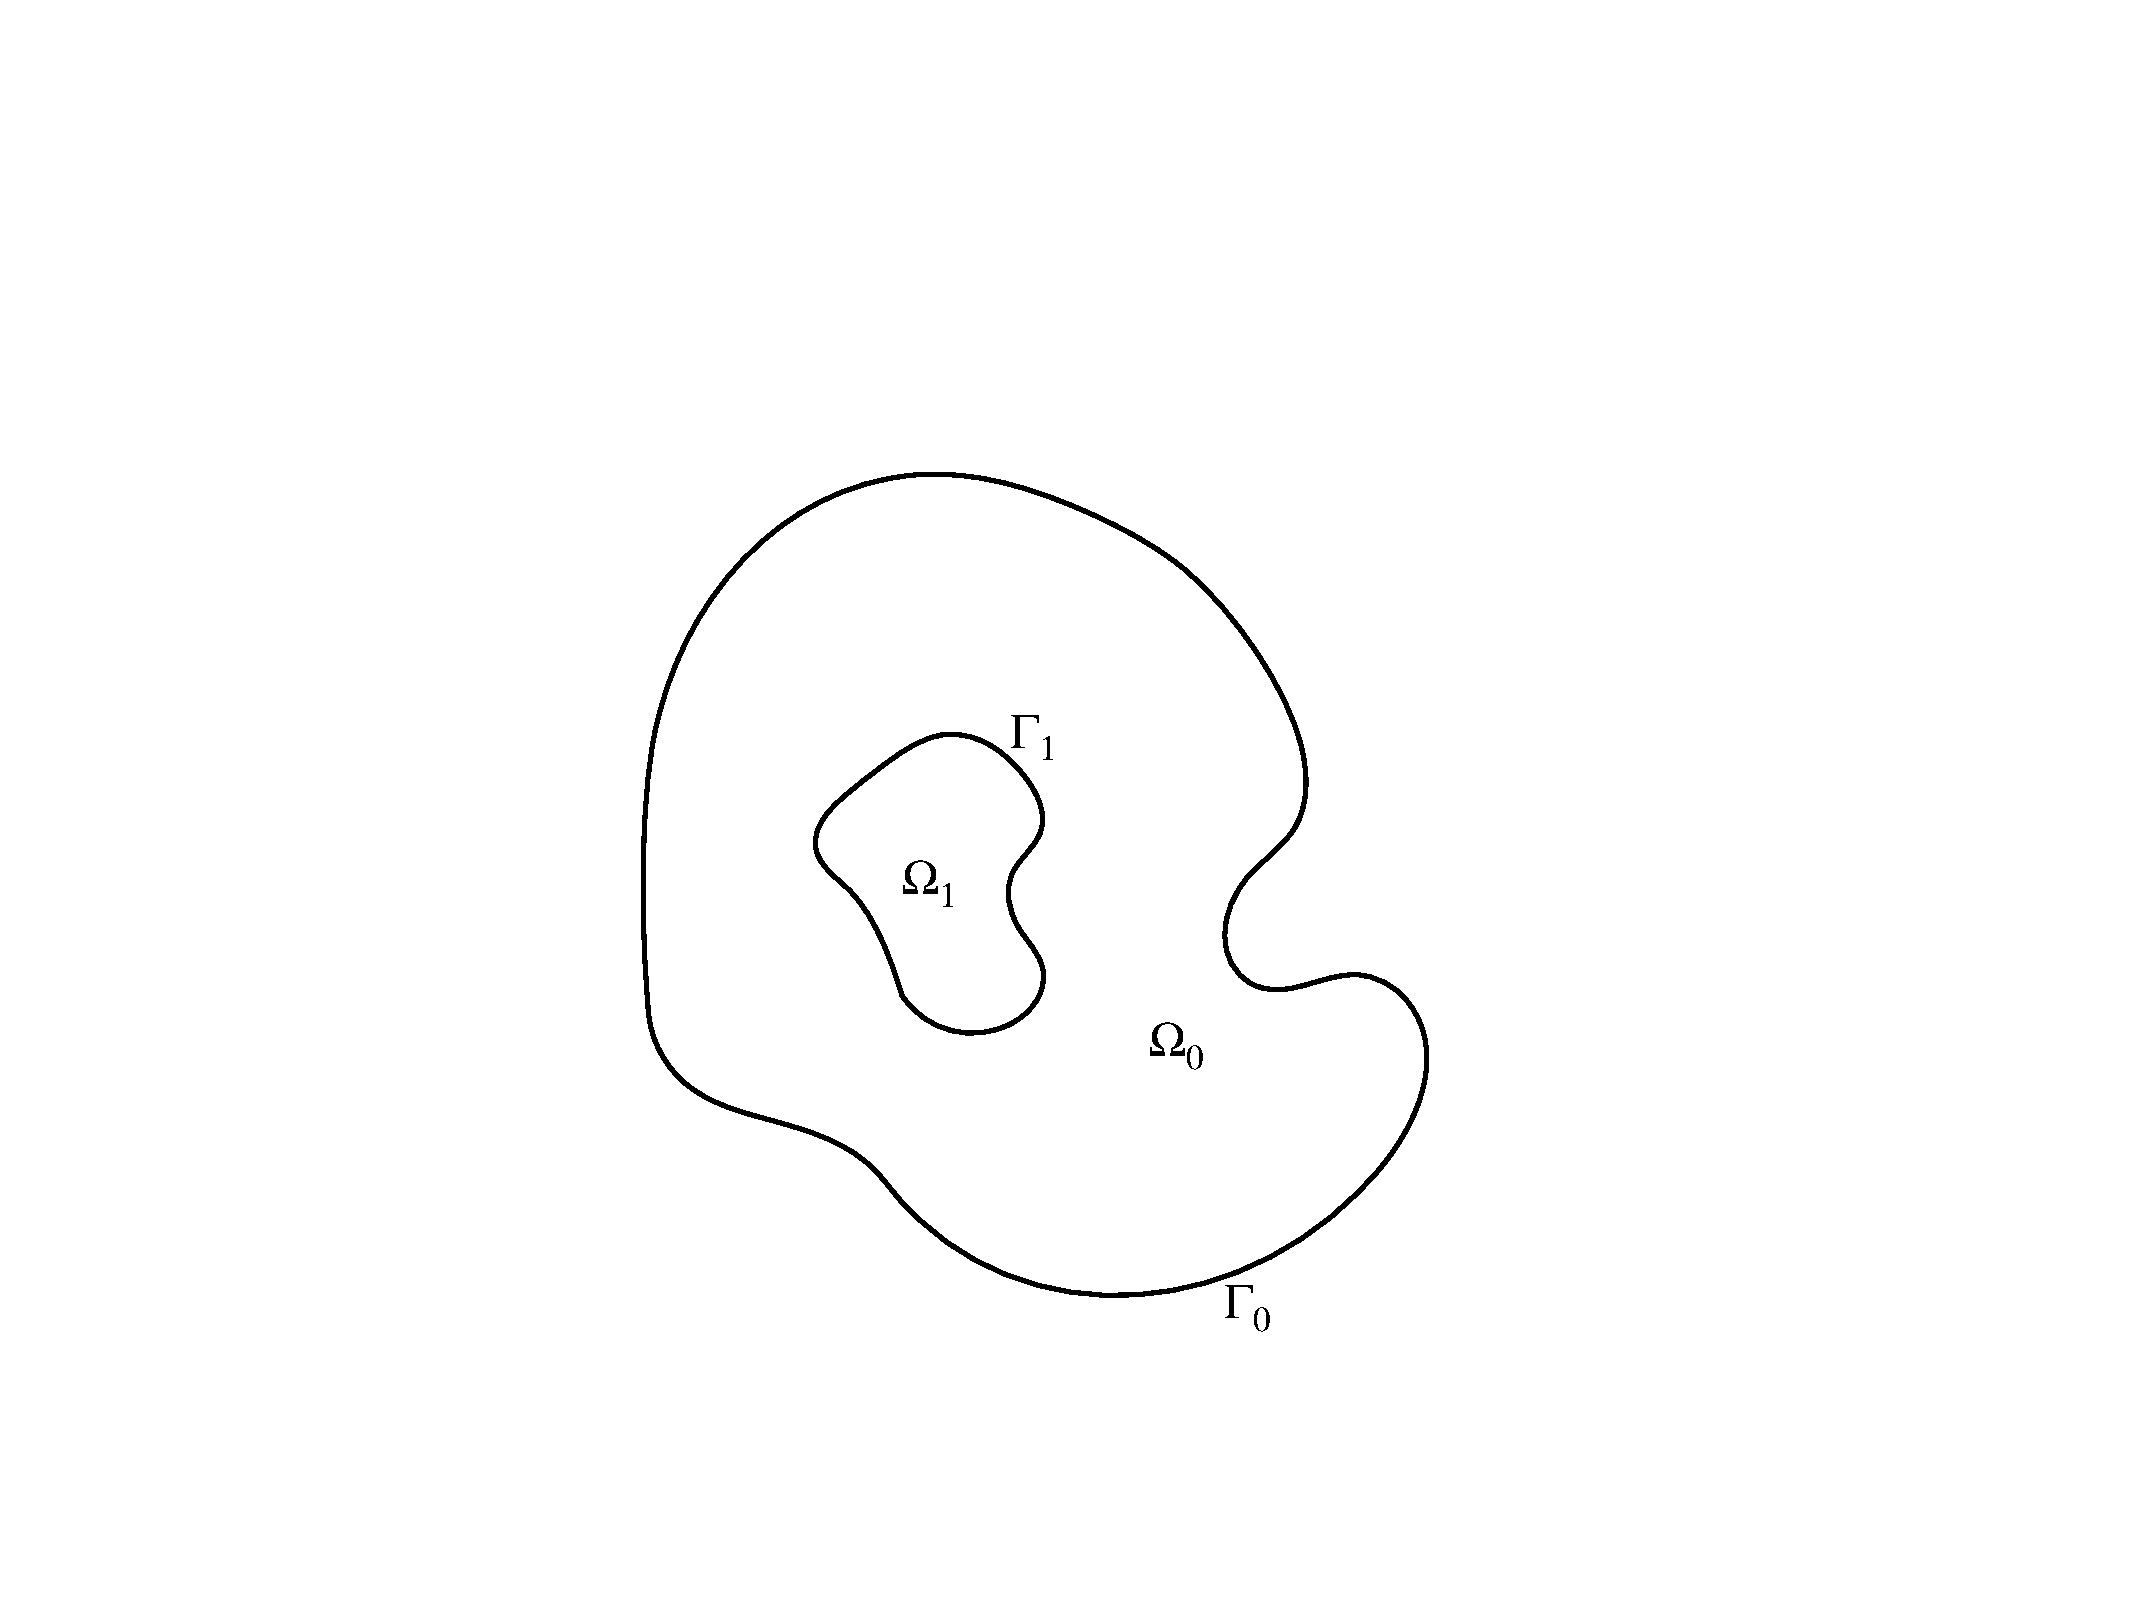
\includegraphics[width=0.3\linewidth]{media/multiply_final}
\end{center}
\caption{Example of a multiply connected domain with one obstacle.}
\label{fig:1ply}
\end{figure}

\begin{proof}
Suppose that $k$ is a Neumann eigenvalue of $\Omega_{1}$. 
$\tilde{\bu}$ be the eigenmode corresponding to this eigenvalue. 
Note that $\tilde{\bu}$ is not identically $0$ on the boundary $\Gamma_{1}$
of $\Omega_{1}$.
Since $\tilde{\bu}$ is an interior Neumann eigenfunction, we note that
the surface traction corresponding to the solution $\bt^{-} = 0$
on the boundary.
Applying Green's identity~\cref{thrm:rep-theorem}, to the solution 
$\tilde{\bu}$ in the interior and taking the interior limit we get
\begin{equation}
\tilde{\bu} = \frac{1}{2}\tilde{\bu} + \cD^{\Gamma_{1}}_{k}[\tilde{\bu}] +
\cS^{\Gamma_{1}} [\bt^{-}] \implies \frac{1}{2} \tilde{\bu} - \cD^{\Gamma_{1}}_{k}[\tilde{\bu}]
= 0\, .
\end{equation}
Note that the sign of the $\bD$ in the representation theorem is switched
since the normal is pointing inwards for the boundary $\Omega_{1}$.
Thus, $\tilde{\bu}$ is a non-trivial null vector of the operator 
$\frac{1}{2}\cI - \cD^{\Gamma_{1}}_{k}$. 
Furthermore since $\tilde{\bu}$ is the boundary data of 
the solution of the oscillatory Stokes equation in $\Omega_{1}$, we
get that $\cW^{\Gamma_{1}}[\tilde{\bu}] = 0$.
Setting $\bmu = \tilde{\bu}$ on $\Gamma_{1}$, and $\bmu = 0$ on $\Gamma_{0}$,
we obtain a non-trivial null vector for the operator $\cI - 2\cD^{\Gamma}_{k} -2\cW^{\Gamma}$
on the boundary $\Gamma = \Gamma_{0} \cup \Gamma_{1}$.
\end{proof}

As noted in~\cite{zhao2015robust}, this lack of one-to-one correspondance between
the invertibility of the integral operator $\cI - 2\cD_{k} - 2\cW$
and the Dirichlet eigenvalues of the Stokes operator on multiply
connected domains causes non-robustness and introduces near 
resonanaces for simply connected domains
which are almost multiply connected.
We demonstrate this issue numerically in~\cref{sec:numanalysis-nearly-mult-con}.

\subsubsection{Mixed layer potential representation}
\label{subsec:mixedanalysis}
The non-robustness of the double layer potential representation
for computing the Dirichlet eigenvalues of Stokes equation can be remdied
by the standard approach of using the mixed layer potential representation,
i.e. setting
$\bu = (\bD_{k} + i\eta \bS_{k})
\bmu$, 
where $\bmu$ is the unknown density to be solved for, and $\eta \in \mathbb{R}^{+}$ 
On imposing the boundary conditions and using~\cref{lem:jump-conds}, 
we obtain the following integral equation on the boundary 
\begin{equation}
(\cI - 2\cD_{k} - 2i\eta \cS_{k}) \bmu = -2 \ff \, . 
\end{equation}
As noted in~\cref{subsubsec:nullspacecorr}, this integral equation 
is also rank-deficient, and we instead use the following 
equivalent integral equation for $\bmu$,
\begin{equation}
(\cI - 2\cD_{k} -2i\eta \cS_{k}  -2\cW)\bmu = -2 \ff \, .
\end{equation}

We now prove that for any bounded region $\Omega$ (simply or multiply
connected) with $C^{2}$ boundaries, there exists a one-to-one correspondance
between the invertibility of the operator
$\cI - 2\cD_{k} - 2i\eta \cS_{k} - 2\cW$ and the Dirichlet eigenvalues
of the Stokes operator on $\Omega$. 

\begin{thrm}
Suppose $\Omega$ is a bounded region defined by the intersection of a 
simply connected domain $\Omega_{0}$ and the exteriors of a finite collection
of bounded simply connected domains $\{ \Omega_{i} \}_{i=1}^{m}$.
As before let $\Gamma_{i}$ denote the boundary of $\Omega_{i}$ and let
$\Gamma = \cup_{i=0}^{m} \Gamma_{i}$ denote the boundary of $\Omega$.
Then the operator $\cI - 2\cD_{k} - 2i\eta \cS_{k} - 2\cW$
is invertible if and only if $k$ is not a Dirichlet eigenvalue
for the Stokes operator on $\Omega$.
\end{thrm}

\begin{proof}
Suppose that $k$ is not a Dirichlet eigenvalue for Stokes equation on
$\Omega$. 
Suppose further that $\bmu$ satisfies
\begin{equation}
(\cI - 2\cD_{k} -2i\eta\cS_{k} - 2\cW) \bmu = 0 \, , \label{eq:mlproofrep}
\end{equation}
i.e. $\bmu$ is in the null-space
of $(\cI - 2 \cD_{k} - 2i\eta \cS_{k} - 2 \cW)$. 
Applying the operator $\cW$ to~\cref{eq:mlproofrep} and 
using~\cref{lem:propnullspacecorr}, we get
\begin{equation}
0 = \cW [(\cI - 2\cD_{k} - 2i\eta\cS_{k} - 2\cW)\bmu] = -2\cW [\bmu] \, .
\end{equation}
Thus~\cref{eq:mlproofrep} reduces to
\begin{equation}
(\cI - 2 \cD_{k} - 2i\eta \cS_{k})\bmu = 0\, .
\end{equation}
Suppose now $\bu = -2\bD_{k}[\bmu] -2i\eta\bS_{k}[\bmu]$ in $\Omega$.
Then $\bu$ is a solution to the oscillatory Stokes equation in $\Omega$,
and applying~\cref{lem:jump-conds}, we get that the interior
limit of the velocity $\bu^{-} = (\cI - 2\cD_{k} -2i\eta\cS_{k}) \bmu = 0$ on $\Gamma$. 
Since $k$ is not a Dirichlet eigenvalue for the Stokes equation on 
$\Omega$, we conclude that $\bu \equiv 0$ in $\Omega$. 
This in particular implies that the interior limit of the surface traction
denoted by $\bt^{-} = 0$ on $\Gamma$.
Using~\cref{lem:jump-conds}  
we observe that the exterior limit 
of the surface traction is $\bt^{+} = i\eta \bmu(\xx)$
and the exterior limit of the velocity is 
$\bu^{+} = \bmu(\xx)$ on $\Gamma$.
\begin{remark}
Note that there is a slight abuse of notation here for the obstacle
boundaries, since the exterior limit with respect to $\Omega$ 
for the boundary $\Gamma_{j}$ is the traditional interior 
limit with respect to the obstacle region $\Omega_{j}$.
\end{remark}
We first show that $\bmu=0$ on $\Gamma_{0}$. 
To this end, note that $\bu$ is a radiating solution of the oscillatory
Stokes equation in the exterior $E$,
since $\cW[\bmu] = 0$ implies that $\int_{\Gamma} \bmu \cdot \bnu = 0$. 
From uniqueness of the impedance problem in the exterior $E$, we conclude
that $\bu \equiv 0$ in $E$ as well, which in particular implies that
the exterior limit of the velocity $\bu^{+}=0$ on $\Gamma_{0}$.   
Using the jump conditions in~\cref{lem:jump-conds} again, we
get that $\bmu = \frac{1}{2}(\bu^{+} - \bu^{-}) = 0$ \, on
$\Gamma_{0}$. 
To show that $\bmu=0$ on $\Gamma_{j}$, we observe that
$\bmu$ is also a solution to the oscillatory Stokes equation
in each of the obstacles $\Omega_{j}$ as well.
Applying Green's identity and using the fact that 
the interior limits with respect to $\Omega_{j}$ (see remark)
of the surface traction and the velocity
are $i\eta \bmu$ and $\bmu$ respectively, we get
\begin{equation}
\int_{\Omega_{j}} (|e(\bu)|^{2} - \overline{k}^{2} |\bu|^2) dV 
= \int_{\Gamma_{j}} \bu \cdot \overline{\bt} dS = 
i\overline{\eta}\int_{\Gamma_{j}} |\bmu|^2 dS \, .
\end{equation}
Taking the imaginary part of the above equation, we get
\begin{equation}
2 \text{Re}(k) \text{Im}(k) \int_{\Omega_{j}} |\bu|^2 + \text{Re}(\eta)
\int_{\Gamma_{j}} |\bmu|^2 dS = 0 \, .
\end{equation}
Since $\text{Re}(\eta)>0$, this implies that $\bmu=0$ for $\xx \in \Gamma_{j}$, $j=1,2,\ldots m$. 
Thus $\cI - 2\cD_{k} -2i\eta\cS_{k} -2\cW$ is invertible when $k$ 
is not a Dirichlet eigenvalue for the Stokes equation on $\Omega$.


From Green's representation for the oscillatory Stokes equation, 
we know that 
  \begin{equation} \label{eq:rep-theorem}
    \bS [\bt](\xx) - \bD[\bu](\xx) = \begin{cases} 
    \bu(\xx) &\quad \xx \in \Omega \, , \\
    0 &\quad \xx \in \Omega^{C} \; .
    \end{cases}
  \end{equation}
Suppose that $k$ is Dirichlet eigenvalue for the Stokes equation on $\Omega$
and let $\bu$ denote the corresponding eigenfunction and let $\bt$ denote
the surface traction associated with the eigenfunction.
Note that the Green's representation theorem implies that 
$\cS_{k}[\bt^{-}] = 0$, since $\bu^{-}=0$ on $\Gamma$. 
Applying the Green's theorem to the pair $\bt^{-}, \bu^{-}$ and taking 
its derivative on $\Gamma$ using~\cref{lem:jump-conds}, we get
\begin{equation}
\bt^{-} = (\cDt_{k} + \frac{1}{2} \cI) \bt^{-} \, . 
\end{equation}
Combining these two identities, we get
that
\begin{equation}
(-\cI - 2\cD_{k} -2i\eta \cS_{k}) \bt^{-} = 0 \, .
\end{equation}
As in the proof of~\cref{thm:dlmain}, letting $c = \left< \bt^{-} ,\bnu \right>$, 
it follows that
\begin{equation}
(-\cI - 2\cD_{k} - 2i \eta \cS_{k} - 2\cW) (\bt^{-} - c\bnu) = 0 \, ,
\end{equation}
where $\bt^{-} - c\bnu \neq 0$.
Since $\bt^{-} - c\bnu$ is non-trivial, and $i\eta \cS_{k}, \cW$ are self-adjoint ($i\eta \cS_{k}$ 
is self-adjoint since we consider inner products without conjugation), 
it follows from the Fredholm alternative 
that the operator $\cI - 2\cD(k) -2i\eta \cS - 2\cW$ is also not invertible.
\end{proof}

\subsection{Fredholm determinants}
Having established the equivalence between the Dirichlet eigenvalues
for Stokes equation and the invertibility of
the operator $\cI - 2\cD_{k} - 2\cW$ on simply connected domains, in this section
we show how the Fredholm determinant can be as a computational tool for detecting
the non-invertibility of $\cI - 2\cD_{k} - 2\cW$.

Let $\cJ_{1}(X)$ denote the space of trace class operators 
on $X$, where $X$ is a Hilbert space.
$\cJ_{1}$ is a subspace of compact operators on $X$.
Suppose that $A$ is a compact operator, with eigenvalues
$\lambda_{i}, i\in \mathbb{N}$.
Then the operator $A \in \cJ_{1}(X)$ if
$\sum_{i} |\lambda_{i}| < \infty$.
If $A$, is a trace class operator, then  
the Fredholm determinant of the operator $\cI + A$ is defined as
\begin{equation}
\text{det}(\cI +A) = \prod_{i=1}^{\infty} (1+\lambda_{i}) \, .
\end{equation}
It follows from standard results in complex analysis, 
that the Fredholm determinant is finite and well-defined if 
$\text{det}(\cI+A) < \infty$ if $\sum_{i} |\lambda_{i}| < \infty$,
i.e. if $A$ is in trace class.

The following lemma shows that the operator 
$-2\cD_{k} - 2\cW$ is a trace class operator.
\begin{lemma} 
$-2\cD_{k} - 2\cW$ is a trace class operator for all $k$ 
\end{lemma}
\begin{proof}
Using Bessel function asymptotics, we note that the
kernel of $\cD_{k}$ given by
$\TT_{\cdot,\cdot,\ell}\nu_{\ell}(\bx,\by)$
has a leading order singularity of $|\bx-\by|^2 \log{|\bx-\by|^2}$ as $\bx\to \by$.
It follows from~\cite{bornemann2010numerical} numerical that $\cD_{k}$
is a trace-class operator for all $k$.
Since $\cW$ is a rank-one perturbation independent of $k$, and trace-class
operators are a vector space, we conclude that
$-2\cD_{k} - 2\cW$ is also a trace-class operator for all $k$.
\end{proof}

Let $f(k) = \text{det}(\cI - 2\cD_{k} - 2\cW)$.
We first note that $f(k)$ is an analytic function of $k$
for $k \in \mathbb{C} \setminus 0$
since the kernel of $\cD_{k}$ is an 
analytic function of $k$ on that domain, 
and the Fredholm determinant is an analytic operator.

The Fredholm determinant of a second-kind Fredholm operator
is another way of detecting when the operator is not invertible. 
The following result summarizes the result. 
\begin{lemma}
$f(k) = 0$ if and only if $\cI - 2\cD_{k} -2\cW$ 
is not invertible.
\end{lemma}
\begin{proof}
The proof is standard and see for example~\cite{simon2005trace}, page 34.
\end{proof}

When $\Omega$ is simply connected, the above lemma combined 
with~\cref{thm:dlmain} implies $f(k) = 0$ if and only if $k$ 
is a Dirichlet eigenvalue for Stokes equation.

We now show how this fact can be used numerically
to estimate the Dirichlet eigenvalues.
Suppose that $M_{k}^{N}$ is a Nystr\"{o}m discretization 
of the operator $-2\cD_{k} - 2\cW$ when the boundary 
$\Gamma$ is discretized with $N$ points. 
Let $f^{N}(k) = \text{det}(I + M_{k}^{N})$
where here $\text{det}$ is the standard matrix determinant.
Note that the discretized matrix also depends on the choice
of quadrature rule used in the Nystr\"{o}m discretization
of the operator.


In~\cite{zhao2015robust}, the authors prove that
for computing the Laplace eigenvalues on regions with 
analytic boundaries, when the integral
operators are discretized using Kress-quadrature~\cite{kress1991boundary},
the determinant of the Nystr\"{o}m discretized operators
at the true eigenvalues converge to $0$ exponentially in $N$.
Thus, if the eigenvalues have multiplicity $1$, i.e. the
derivative of the determinant is non-zero at the true-eigenvalues,
then the analyticity of the discretized determinant implies
that the zeros of the determinant of the Nystr\"{o}m 
discretization of the linear operator converge
exponentially to the true Dirichlet eigenvalues for Laplace's equation.

The proof presented in~\cite{zhao2015robust} carries forward
for computing the Dirichlet eigenvalues of Stokes equation as well.
We summarize the result in the following theorem.
\begin{thrm}
\label{thm:mainconvfreddet}
Suppose that $\Omega$ is a simply connected domain with an analytic boundary.
Let $k_{j}$, $j=1,2,\ldots M$ denote all the Dirichlet eigenvalues of Stokes
equation on $\Omega$ contained in the interval $[a,b]$. 
Suppose further that all the eigenvalues have multiplicity $1$.
Let $f^{N}(k) = \text{det}(I+M^{N}_{k})$, where $M^{N}_{k}$ 
is the Nystr\"{o}m discretzation of $-2\cD_{k} - 2\cW$ with Kress
quadrature.
Then $f^{N}(k)$ has exactly $M$ zeros on the interval $[a,b]$. 
Let $\omega_{j}$, $j=1,2\ldots M$ denote the zeros of $f^{N}$.
Furthermore, there exist constants $a>0$ and $C$, 
such that $\sup_{j=1}^{M} |\omega_{j} - k_{j}| < C e^{-aN}$.
\end{thrm}

\begin{proof}
The proof follows from small modificiations of the proofs contained in~\cite{zhao2015robust}. 
\end{proof}

In practice, using Kress-quadrature for large problems is problematic owing to the global
nature of the quadrature rule. 
The coupling with fast direct solvers for computing determinants also results in $O(N^2 \log{N})$ 
determinant evaluation since evaluating each matrix entry costs $O(N)$, where 
$N$ is the number of discretization points on the boundary.
Over the last two decades, many high-order quadrature methods which are compatible with
fast algorithms like the fast multipole method (and fast direct solvers as well, 
since each matrix entry requires O(1) work) have been developed for solving
integral equations.
Extensive numerical evidence suggests that the zeros of the 
determinants of linear systems discretized using 
these quadrature methods are also high order approximations of Dirichlet eigenvalues
for the Stokes PDE--- the error is observed to be proportional to the quadrature error
for the eigenfunction $\bt^{-}$ associated with the eigenvalue.
We leave a proof of this to future work.


\begin{remark}
The same analysis does not carry through for the operator
$\cI - 2 \cD_{k} - 2i\eta \cS_{k} - 2\cW$, 
since $\cS_{k}$ is not a trace class operator.
For brevity, let $\cM_{k} = -2\cD_{k} - 2i\eta \cS_{k} - 2\cW$.
The operator $\cM_{k}$ is 
in $\cJ_{2}(\bL^{2}(\Gamma))$ where
$\cJ_{2}(\bL^{2}(\Gamma))$ is the space of Hilbert-Schmidt operators
on $\bL^{2}(\Gamma)$ (the singular values of the operator are square
summable, as opposed to being summable).
Thus the Fredholm determinant of $\cI + \cM_{k}$
is not necessarily finite. 
However, as noted in~\cite{zhao2015robust}, the convergence
result~\cref{thm:mainconvfreddet}
should be true up to a logarithmic factor in the rate
of convergence, since the singular values of the operator
$\cM_{k}$ decay like $\frac{1}{n}$, and the
Fredholm determinant divergers logarithmically. 
In~\cref{subsec:convannulus}, we demonstrate that this fact
numerically on the annulus, where the eigenvalues are analytically known. 
\end{remark}
